\documentclass[12pt]{article}

% Packages
\usepackage[margin=1in]{geometry}
\usepackage{amsmath, amssymb}
\usepackage{graphicx}
\usepackage{hyperref}
\usepackage{xcolor}
\usepackage{enumitem}
\usepackage{booktabs}
\usepackage{tcolorbox} % For boxes
\tcbset{colback=gray!10, colframe=black, boxrule=0.5pt, arc=4pt}
\usepackage{graphicx} % For inserting images
\usepackage{caption}  % For customizing captions
\usepackage{xcolor} % for colored text





% Custom Commands
\newcommand{\definition}[2]{
    \begin{tcolorbox}
    \textbf{#1:} #2
    \end{tcolorbox}
}
\newcommand{\formula}[2]{
    \begin{tcolorbox}[colback=blue!5!white]
    \textbf{#1:} \[ #2 \]
    \end{tcolorbox}
}


% Custom "lead words" command
\newcommand{\leadwords}[2]{\textcolor{red}{\textbf{\large #1}} #2}

% Paragraph formatting
\setlength{\parindent}{0pt} % No paragraph indentation
\setlength{\parskip}{0.8em} % Space between paragraphs


\title{Introductory Macroeconomics Notes}
\author{Abdullah Yassine}
\date{\today}

\begin{document}

\maketitle
\tableofcontents
\newpage

\section{The Science of Macroeconomics}
\definition{Macroeconomics}{The study of the economy as a whole, focusing on aggregate measures and national policies.}

\subsection{Theory as Model Building}
Children try to learn how the world around them work by playing with little toys. Similarly, economists try to learn how economies work by playing with \textbf{models}. Models often help economists to try to understand the relationship between variables.



Models have two kinds of variables:
\begin{itemize}
    \item \textbf{Endogenous Variables}: variables that a model tries to explain.
    \item \textbf{Exogenous Variables}: variables a model take as given.
\end{itemize}


In other words, models try to explain how exogenous variables affect endogenous variables. Exogenous variables come from outside the model and act as the model's input, whereas endogenous variables are determined within the model and act as the model's output.



\subsection{Prices: Flexbile Versus Sticky}

When creating models, we make assumptions, and we have to keep those assumptions in mind when we make conclusions based on the model. One of the assumptions we make when creating models is \textbf{market clearing} where we assume that whenever something happens to the supply or demand curve, the equilibrium price changes instantly.


In reality, prices and wages stay the same for a long time before changing. For example, job contracts require to pay the same wage rate for 3 years. Magazine companies sell their magazines at the same price for a couple of months before changing those prices.



Market clearing is the best for long-term modelling, while \textbf{market sticky} is best used in short-term modelling.


\section{The Data of Macroeconomics}
% \definition{Gross Domestic Product (GDP)}{The total market value of all final goods and services produced within a country in a given period.}

% \formula{Nominal GDP}{P_t \times Q_t}
% \formula{Real GDP}{P_{\text{base}} \times Q_t}
Now, we learn the tools that are used by macreconomists so they can have a better understanding of the economy.

\definition{Gross Domestic Product (GDP)}{The total market value of all final goods and services produced within a country in a given period. Another definition includes the total income of everyone in the country.}


How is total income the same thing as output produced by the country? When Jill builds a house and sells it to Joe for \$10,000, it's income for Jill but an expenditure to Joe. Regardless, \$10,000 is now part of the GDP.

To better understand this, let's assume a scenario where the economy only produces one product, bread. In this economy, households sell their labor to the firms. Firms use this labor to produce bread which they sell to households. Firms pay money to households for their labor, and households use that money to buy bread from firms. Look at the following figure.


\begin{figure}[h!]
    \centering
    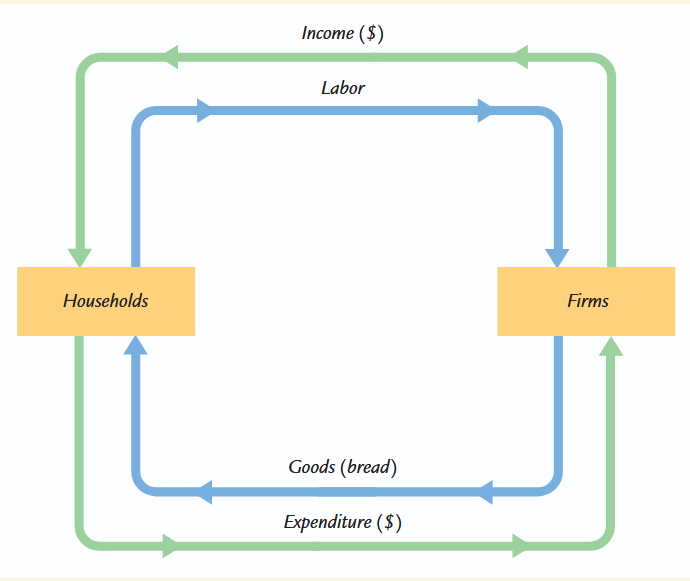
\includegraphics[width=0.75\textwidth]{images/flow.png}
    \caption{The Circular Flow.}
    \label{fig:aggregate_demand}
\end{figure}


So, GDP in this case can be measured in two cases: total income from the production of bread (the top loop), or the total expenditure on purchases of bread (the bottom loop).


\subsection{Rules for Computing GDP}


When an economy gets complicated and starts to sell many stuff, how do we calculate GDP now? Just like before, but this time, we use the \textit{market price} because these prices reflect how much people are willing to pay for a good or service.



\leadwords{Used Goods} When it comes to used goods, like someone reselling a pack of basketball cards, that does not go to the GDP because GDP is all about \textit{currently} produced goods and services. This is just a transfer of assets.


\leadwords{The Treatment of Inventories} Let's assume that the firm now produced more bread, which required hiring more workers and increasing wage rates. But nobody buys the bread, what happens to the GDP? Depeds on what happens to the bread.

If the firm just throws away the bread, then nothing is added to the GDP -- even though wages increased and more workers hired. This is because nothing got sold, and when we say the sum of all income, we mean the sum of all income that come from producing goods and services. In this case, the bread isn't sold.

What happens when the firm put the bread in inventory? In this case, it's assumed that the owners "purchased" the inventory bread, so the additional cost of wages is covered by the owners buying the bread. In this case, it's added to the GDP.

What happens when they later actually sell it? It's just counted as if they sold a used item.

\leadwords{Intermediate Goods and Value Added} If McDonald's buy a quarter pounder from a farmer for \$1, use the meat to produce a burger and sell it for \$4, how should GDP be counted in this case? Should the value added to the GDP be \$5? No, and we should only add the \textit{final} product produced and not the intermediate products.

This is because intermediate goods are already included in the cost of producing the burger, and so it include the double pounder is to double count.

One way to compute the value of all final goods produced is to sum the value added in each stage. The \textbf{value added} equals the value of the firm's output less the value of the intermediate goods. For the farmer, let's say the value added is \$1 (he didn't buy any intermediate goods), and the value added of McDonald's is \$3 - \$1 = \$2. The total is thus \$3.

Thus, GDP can also be counted as the total value added of all firms in the economy.

\leadwords{Housing Services and Other Imputations} Some stuff do not have market prices because they are not sold in marketplaces. \textbf{Imputed value} is the estimate value of these goods so they can be included in the GDP.

For homeowners, the "rent" they pay to themselves is included in the GDP. This is not perfect because, for example, you can have jewelry and the value of it is not in the GDP.

Also, no imputation is made for the stuff sold in \textit{underground economy}.

\subsection{Real GDP Versus Nominal GDP}

What if in year 2, the economy produced the same amount of stuff as last year but the prices increased because of inflation. Because of this, GDP increased. But this is a poor indicator of the health of the economy on whether the economy's ability to satisfy demands because the stuff got produced. This is called \textbf{nominal GDP}, when you account for changes in quantity produced \textit{and} price changes.

A better indicator is \textbf{real GDP}, which measures changes in quantity produced but the prices remain the same.


\subsection{The GDP Deflator}

The \textbf{GDP Deflator} is measured as: $$\text{GDP Deflator } = \frac{\text{Nominal GDP}}{\text{Real GDP}}$$
The deflator reflects what's happening to the overall level of prices in the economy.


\end{document}
